% This is "sig-alternate.tex" V2.1 April 2013
%DIF LATEXDIFF DIFFERENCE FILE
%DIF DEL sig-alternate-sample.tex       Mon Feb 19 15:05:51 2018
%DIF ADD sig-alternate-sample-new.tex   Mon Feb 19 16:01:44 2018
% This file should be compiled with V2.5 of "sig-alternate.cls" May 2012
%
% This example file demonstrates the use of the 'sig-alternate.cls'
% V2.5 LaTeX2e document class file. It is for those submitting
% articles to ACM Conference Proceedings WHO DO NOT WISH TO
% STRICTLY ADHERE TO THE SIGS (PUBS-BOARD-ENDORSED) STYLE.
% The 'sig-alternate.cls' file will produce a similar-looking,
% albeit, 'tighter' paper resulting in, invariably, fewer pages.
%
% ----------------------------------------------------------------------------------------------------------------
% This .tex file (and associated .cls V2.5) produces:
%       1) The Permission Statement
%       2) The Conference (location) Info information
%       3) The Copyright Line with ACM data
%       4) NO page numbers
%
% as against the acm_proc_article-sp.cls file which
% DOES NOT produce 1) thru' 3) above.
%
% Using 'sig-alternate.cls' you have control, however, from within
% the source .tex file, over both the CopyrightYear
% (defaulted to 200X) and the ACM Copyright Data
% (defaulted to X-XXXXX-XX-X/XX/XX).
% e.g.
% \CopyrightYear{2007} will cause 2007 to appear in the copyright line.
% \crdata{0-12345-67-8/90/12} will cause 0-12345-67-8/90/12 to appear in the copyright line.
%
% ---------------------------------------------------------------------------------------------------------------
% This .tex source is an example which *does* use
% the .bib file (from which the .bbl file % is produced).
% REMEMBER HOWEVER: After having produced the .bbl file,
% and prior to final submission, you *NEED* to 'insert'
% your .bbl file into your source .tex file so as to provide
% ONE 'self-contained' source file.
%
% ================= IF YOU HAVE QUESTIONS =======================
% Questions regarding the SIGS styles, SIGS policies and
% procedures, Conferences etc. should be sent to
% Adrienne Griscti (griscti@acm.org)
%
% Technical questions _only_ to
% Gerald Murray (murray@hq.acm.org)
% ===============================================================
%
% For tracking purposes - this is V2.0 - May 2012

\documentclass{sig-alternate-05-2015}
%DIF PREAMBLE EXTENSION ADDED BY LATEXDIFF
%DIF UNDERLINE PREAMBLE %DIF PREAMBLE
\RequirePackage[normalem]{ulem} %DIF PREAMBLE
\RequirePackage{color}\definecolor{RED}{rgb}{1,0,0}\definecolor{BLUE}{rgb}{0,0,1} %DIF PREAMBLE
\providecommand{\DIFadd}[1]{{\protect\color{blue}\uwave{#1}}} %DIF PREAMBLE
\providecommand{\DIFdel}[1]{{\protect\color{red}\sout{#1}}}                      %DIF PREAMBLE
%DIF SAFE PREAMBLE %DIF PREAMBLE
\providecommand{\DIFaddbegin}{} %DIF PREAMBLE
\providecommand{\DIFaddend}{} %DIF PREAMBLE
\providecommand{\DIFdelbegin}{} %DIF PREAMBLE
\providecommand{\DIFdelend}{} %DIF PREAMBLE
%DIF FLOATSAFE PREAMBLE %DIF PREAMBLE
\providecommand{\DIFaddFL}[1]{\DIFadd{#1}} %DIF PREAMBLE
\providecommand{\DIFdelFL}[1]{\DIFdel{#1}} %DIF PREAMBLE
\providecommand{\DIFaddbeginFL}{} %DIF PREAMBLE
\providecommand{\DIFaddendFL}{} %DIF PREAMBLE
\providecommand{\DIFdelbeginFL}{} %DIF PREAMBLE
\providecommand{\DIFdelendFL}{} %DIF PREAMBLE
%DIF END PREAMBLE EXTENSION ADDED BY LATEXDIFF

\begin{document}

% Copyright
\setcopyright{acmcopyright}
%\setcopyright{acmlicensed}
%\setcopyright{rightsretained}
%\setcopyright{usgov}
%\setcopyright{usgovmixed}
%\setcopyright{cagov}
%\setcopyright{cagovmixed}


% DOI
\doi{10.475/123_4}

% ISBN
\isbn{123-4567-24-567/08/06}

%Conference
\conferenceinfo{PLDI '13}{June 16--19, 2013, Seattle, WA, USA}

\acmPrice{\$15.00}

%
% --- Author Metadata here ---
\conferenceinfo{WOODSTOCK}{'97 El Paso, Texas USA}
%\CopyrightYear{2007} % Allows default copyright year (20XX) to be over-ridden - IF NEED BE.
%\crdata{0-12345-67-8/90/01}  % Allows default copyright data (0-89791-88-6/97/05) to be over-ridden - IF NEED BE.
% --- End of Author Metadata ---

\title{MoViMash: Online Mobile Video Mashup}


%\subtitle{[Extended Abstract]
%\titlenote{A full version of this paper is available as
%\textit{Author's Guide to Preparing ACM SIG Proceedings Using
%\LaTeX$2_\epsilon$\ and BibTeX} at
%\texttt{www.acm.org/eaddress.htm}}}


%
% You need the command \numberofauthors to handle the 'placement
% and alignment' of the authors beneath the title.
%
% For aesthetic reasons, we recommend 'three authors at a time'
% i.e. three 'name/affiliation blocks' be placed beneath the title.
%
% NOTE: You are NOT restricted in how many 'rows' of
% "name/affiliations" may appear. We just ask that you restrict
% the number of 'columns' to three.
%
% Because of the available 'opening page real-estate'
% we ask you to refrain from putting more than six authors
% (two rows with three columns) beneath the article title.
% More than six makes the first-page appear very cluttered indeed.
%
% Use the \alignauthor commands to handle the names
% and affiliations for an 'aesthetic maximum' of six authors.
% Add names, affiliations, addresses for
% the seventh etc. author(s) as the argument for the
% \additionalauthors command.
% These 'additional authors' will be output/set for you
% without further effort on your part as the last section in
% the body of your article BEFORE References or any Appendices.

\numberofauthors{4} %  in this sample file, there are a *total*
% of EIGHT authors. SIX appear on the 'first-page' (for formatting
% reasons) and the remaining two appear in the \additionalauthors section.
%
\author{
% You can go ahead and credit any number of authors here,
% e.g. one 'row of three' or two rows (consisting of one row of three
% and a second row of one, two or three).
%
% The command \alignauthor (no curly braces needed) should
% precede each author name, affiliation/snail-mail address and
% e-mail address. Additionally, tag each line of
% affiliation/address with \affaddr, and tag the
% e-mail address with \email.
%
% 1st. author
\alignauthor
Mukesh Saini\\
       \affaddr{Dept. of Computer Science}\\
       \affaddr{National University of Singapore}\\
       \email{mksaini@comp.nus.edu.sg}
% 2nd. author
\alignauthor
Raghudeep Gadde\\
       \affaddr{Dept. of ECE}\\
       \affaddr{National University of Singapore}\\
       \email{elerdg@nus.edu.sg}
% 3rd. author
\and  % use '\and' if you need 'another row' of author names
% 4th. author
\alignauthor
Shuicheng Yan\\
       \affaddr{Dept. of ECE}\\
       \affaddr{National University of Singapore}\\
       \email{eleyans@nus.edu.sg}
\alignauthor
Wei Tsang Ooi\\
       \affaddr{Dept. of Computer Science}\\
       \affaddr{National University of Singapore}\\
       \email{ooiwt@comp.nus.edu.sg}
}
% There's nothing stopping you putting the seventh, eighth, etc.
% author on the opening page (as the 'third row') but we ask,
% for aesthetic reasons that you place these 'additional authors'
% in the \additional authors block, viz.
%\additionalauthors{Additional authors: John Smith (The Th{\o}rv{\"a}ld Group,
%email: {\texttt{jsmith@affiliation.org}}) and Julius P.~Kumquat
%(The Kumquat Consortium, email: {\texttt{jpkumquat@consortium.net}}).}
%\date{30 July 1999}
% Just remember to make sure that the TOTAL number of authors
% is the number that will appear on the first page PLUS the
% number that will appear in the \additionalauthors section.

\maketitle
\begin{abstract}
With the proliferation of mobile video cameras, it is becoming easier
for users to capture videos of live performances and socially
share them with friends and public. As an attendee of such live
performances typically has limited mobility, each video camera is
able to capture only from a range of restricted viewing angles and
distance, producing a rather monotonous video clip. At such performances,
however, multiple video clips can be captured by different
users, likely from different angles and distances. These videos
can be combined to produce a more interesting and representative
mashup of the live performances for broadcasting and sharing. The
earlier works select video shots merely based on the quality of currently
available videos. In real video editing process, however, recent
selection history plays an important role in choosing future
shots. In this work, we present MoViMash, a framework for automatic
online video mashup that makes smooth shot transitions to
cover the performance from diverse perspectives. Shot transition
and shot length distributions are learned from professionally edited
videos. Further, we introduce view quality assessment in the framework
to filter out shaky, occluded, and tilted videos. To the best
of our knowledge, this is the first attempt to incorporate historybased
diversity measurement, state-based video editing rules, and
view quality in automated video mashup generations. Experimental
results have been provided to demonstrate the effectiveness of
MoViMash framework.\\
\textbf{Categories and Subject Descriptors:}
I.2.10 [Vision and Scene
Understanding]: Video Analysis\\
\textbf{General Terms:}
Algorithms, Design.\\
\textbf{Keywords:}
Mobile Video, Virtual Director, Video Mashup.\\
\end{abstract}


\section{Introduction}
Worldwide shipment of camera phones were estimated to reach
1.14 billion in the year 2011 alone [1]. Furthermore, a survey of
over 2,500 respondents by Photobucket reveals that 45\% of the respondents use mobile devices to shoot video at least once weekly during the summer of 2011, validating the significant increase in the amount of mobile video uploaded to Photobucket’s video sharing website (14×in Summer 2011 compared to December 2010) [2].

Proliferation of such mobile devices with video capture capability has enabled users to capture video of their life events such as concerts, parades, outdoor performances, etc, and socially share them with friends and public as it happens. \DIFdelbegin \DIFdel{Videos recorded by a single user at such events are shot from a limited range of angles and distances from the performance stage, as an attendee typically has limited mobility (e.g., constraint by seating arrangement). The recorded video can be monotonous and uninteresting. Furthermore, videos recorded are typically short (in the order of minutes or tens of minutes), due to tired arms or power constraint of mobile devices. There are, however, likely to have more than one users recording the same performance from different angles }\DIFdelend \DIFaddbegin \DIFadd{Vidifferent angles }\DIFaddend at the same time, especially at a well-attended performance.

These recorded and shared video clips of the same performance can be cut and joined together to produce a new mashup video, similar to how a TV director of a live TV show would switch between different cameras to produce the show. Generation of a \DIFdelbegin \DIFdel{video }\DIFdelend \DIFaddbegin \DIFadd{videedhwjhbwjehfbjeo }\DIFaddend mashup can be cast as a video selection problem: given a set of video clips capturing the same performance event, automatically select one of the video clips at any one time instance to be included in the output mashup video.

In this paper, we introduce MoViMash, our approach to solve the above video selection problem. MoViMash aims to produce mashup video from a set of mobile devices that is interesting and pleasing to watch, and uses a combinations of content-analysis, state-based transitions, history-based diversity, and learning from human editors to achieve this goal.

We now provide an overview of how MoViMash works in the usual setting of live performances, shown in Figure 1. There is generally a staging area and an audience area where the audiences either sit or stand to watch the performance, and record the performance with a mobile device. This setting poses a few challenges to video mashup.

Since the videos are recorded with a hand-held mobile device, from the audience area, and likely by non-professional, there is no guarantee on the view quality. The videos can be shaky or tilted. Furthermore, it is common to include the back of the head of other audiences in the view. As other audiences move, the view can be temporarily occluded. When MoViMash needs to decide which video to select, it first filters out the videos with bad views currently from further consideration for selection. To achieve this, MoVi-Mash analyzes the video to determine the current shakiness, the tilt angle, and the level of occlusion in the video. Note that shakiness and tilt angle can be obtained from easily sensory data of mobile device when available.

The shooting angle of the remaining videos are then classified as either center, left, and right; and distance from the stage as near and far as shown in Figure 1. This classification is done every time we perform video selection because mobile users may change their position over time. MoViMash now decides which shooting angle and distance should be used; and for how long the selected class should persist. To this end, MoViMash tries to imitate a professional video editor, by using a finite state machine, whose transition probabilities are learned from analyzing professionally edited videos of the same type of event. The rationale behind the inclusion of learning is that, we have observed that there are no generic editing rules that can be precisely defined to work with all types of events. The video editors make fine decisions such as shot lengths and transitions based on their experience which is hard to enumerate.

The videos from the selected class are further ranked based on the video quality and diversity values to make the final selection. To consider video quality, MoViMash favors video with low blurriness, low blockiness (good compression), good contrast, and good illumination in each video. To consider diversity, MoViMash stores a history of recent video selections and favors videos with dissimilar views with recent selections.

We have developed MoViMashΓÇÖs algorithm such that it is online and only depends on history information. As such, even though it is not our main goal in this paper, MoViMash can be applied to mashup of live video feeds from mobile devices.

We now briefly compare MoViMash to existing work to highlight the contribution of this paper. There has been few works on video selection in a lecture broadcast and video streaming [21] [6] and video conferencing [3]. In these works the camera is mainly selected based on speaker detection. Live performances are not speaker centric. In fact, the speech signals are generally noise from the crowd. In one recent work, Shrestha et al. [15] propose a method to create a video mashup from a given set of concert recordings. In that work, the authors select the shots based on mainly video quality, mostly ignoring view quality. Also, the diversity is only calculated based on the comparison of the last image of the current shot and first image of the next shot. It does not consider the history of video selection and the time for which a particular camera is selected. Further, video editing rules, which are subtle in the case of live performances, are not considered.

\textbf{Contributions.}
We now summarize our contributions in this paper
as follows:
\begin{itemize}
\item We propose a state-based approach for shot selection that incorporates the selection history in the decision process. Earlier methods select shots based on only currently available videos.
\item We include view quality in the framework to filter out the bad views that are occluded, tilted, or shaky. Earlier methods only considered video quality.
\item We build a comprehensive model to calculate diversity that considers both previously selected videos and shot lengths.
\item We propose a learning-based approach where the shot transition probabilities and shot lengths are learned from professionally edited videos.
\end{itemize}

\textbf{Organization.}
The rest of the paper is organized as follows.\\
We provide a review of earlier work in Section 2. In Section 3 we describe proposed mashup framework. We evaluate our system in Section 4. The conclusions are provided in Section 5.

\DIFaddbegin 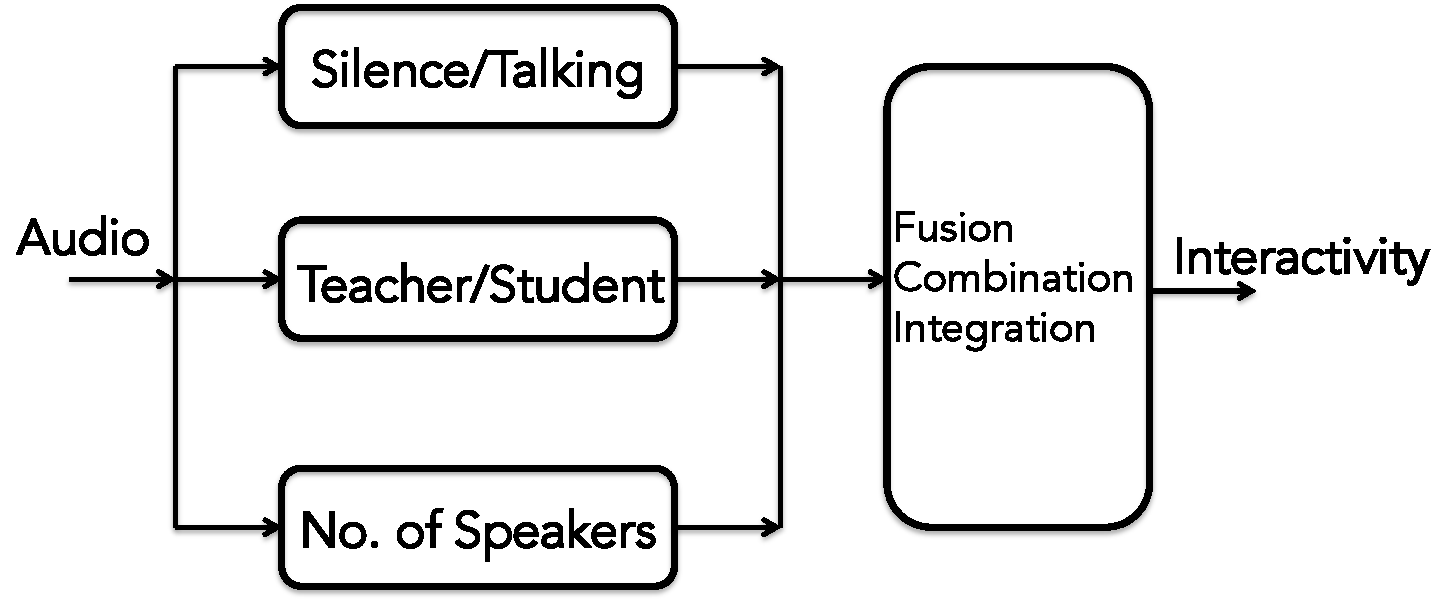
\includegraphics[width=3in]{block-diagram.pdf}

\DIFaddend \section{PREVIOUS WORK}
There has been only few works on online camera selection. In
most of these works, videos are mainly selected to show the speakers.
In the work by Machnicki and Rowe [9], an online lecture
webcast system is presented in which the cameras that are focusing
on speaker and the presentation (the screen) are selected iteratively
until anybody from audience asks question. When audience ask
question, the camera that is focusing the person asking question is
selected. The automatic selection of cameras in a lecture webcast
is extended by Zhang et al. [21] to \DIFdelbegin \DIFdel{include audio based localization
and speaker tracking. Similar approach is taken by Cutler et al. }%DIFDELCMD < [%%%
\DIFdel{6}%DIFDELCMD < ]
%DIFDELCMD < %%%
\DIFdel{in a meeting scenario where camera that shows the current speaker
is selected. Ranjan et al. }%DIFDELCMD < [%%%
\DIFdel{12}%DIFDELCMD < ] %%%
\DIFdel{use face tracking and audio analysis
to show the close-up of the person talking. Since performers
play more important role than speakers in live concerts}\DIFdelend \DIFaddbegin \DIFadd{incmnedjebdkqwjdkwb3i2uedincerts}\DIFaddend , a speaker
based selection is not appropriate. Further, the faces are generally
far from the camera which cannot be detected. Therefore, face detection
is not a reliable basis to select videos.

Al-Hames et al. [3] extends the camera selection work to include
the motion features. We do not use motion features in our framework
because both performers and audience generate continuous
motion. Also, the movement of the mobile camera can inject erroneous
motion in the video, which is aesthetically appealing. Yu et
al. [20] propose to customize the camera selection and shot lengths
based on user preferences. At every lecture webcast receiving site,
the user can give score to the videos and specify rules for shot
lengths. While such an interactive selection of cameras is useful
for educational scenarios, people may find it annoying and stressful
for performances, particularly when the number of videos is
large.

A camera selection method for sports video broadcast is proposed
by Wang et al. [16]. The authors assume one main camera
and other sub cameras. The empirical main camera duration is
found to be from 4 to 24 seconds, and sub camera duration is found
to be 1.5 to 8 seconds. They select a sub camera based on the clarity
of the view, determined using motion features. In our work,
along with shakiness of the videos, we also calculate view quality
in terms of occlusion and rotation; and video quality in terms
of contrast, blur, illumination, and blockiness. We also include
explicit measurement of diversity in the framework. Engstrom et
al. [8] discuss automatic camera selection for broadcast in a sports
event capture scenario. The work mainly promotes collaborative
video production, i.e., video recorded by production team as well
as the consumers.

In other media production applications, the shots are selected to
convey the story to the audience. For instance, de Lima et al. [7] propose a method to automatically select shots from multiple cameras
for storytelling, according to the rules provided by the director.
These methods are not useful for us as live performances generally
do not have any story.

Recently, there has been works on creating video mashups from
given set of videos. In one of the most recent works [15], Shrestha
et al. select the cameras based on video quality. Although the authors
refer to term ΓÇÿdiversityΓÇÖ in the paper, it is merely a comparison
of current frame and the next frame of the corresponding camera.
The authors completely ignore the selection history and the
time for which each view is selected. The authors also ignore editing
rules corresponding to different views, which we incorporate
through learning based classification and selection. Furthermore,
unlike the method proposed in this paper, the authors rely on the
future video for current shot selection. While this approach is fine
for combining stored videos, it is not suitable for live applications
such as broadcasting and live sharing.

We have provided a comparison of the related work in Table 1.
The works have been compared with respect to the following aspects:
(1) can the method be applied online (a method that uses future
information cannot be applied online)? (2) is selection historybased
diversity considered? (3) is learning incorporated? (4) is
video quality (clarity, contrast etc.) considered? (5) is view quality
(view occlusion, tilted view etc.) considered? and (6) what is the
underlying application scenario? It can be easily seen that the proposed
method is the first attempt to consider history based diversity
through learning for online video selection for live performances.

\section{MOVIMASH FRAMEWORK}
In this section, we first enumerate the design principles that we
have followed in the development of \DIFdelbegin \DIFdel{MoViMash }\DIFdelend \DIFaddbegin \DIFadd{MoViMashe3112 }\DIFaddend and then describe
the framework. After an overview of MoViMash, we focus on individual
components.
\DIFaddbegin 

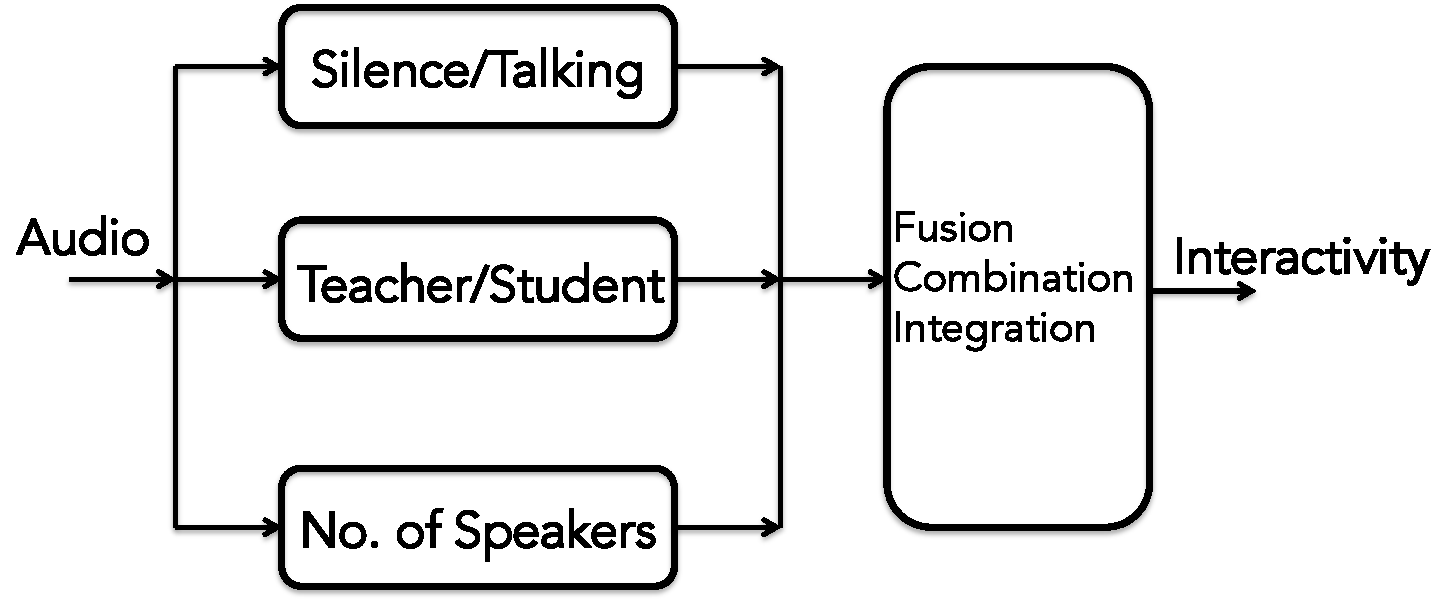
\includegraphics[width=3in]{block-diagram.pdf}
\DIFaddend 

\subsection{Design Principles}
The end goal of the MoViMash is to produce a mashup that users
like. To achieve this goal, we have followed a set of design principles
as follows:

\begin{itemize}
\item \textbf{Video Quality:}
In our discussion, video quality includes
sharpness, contrast, illumination, and blockiness (due to video
compression). A good image quality gives pleasing experience
to the viewers [10]. Therefore, in our framework we
give priority to good quality videos.
\item \textbf{View Quality:}
A video that is captured by a tilted camera
(rotated around horizontal axis) may have very good video
quality, yet, users generally do not like tilted views. Similarly,
a view in which a person or object is occluding stage
area (blocking performance view) may be annoying to the user. Therefore view quality is also important. We measure
view quality in terms of occlusion, tilt, and shakiness.
\item \textbf{Diversity:}
While static cameras always record videos from
same perspective, mobile users generally shoot videos from
a number of views and diverse perspectives. We take this
opportunity to include more diversified views in the mashup.
Both temporal and spatial aspects of diversity are considered
in the proposed framework.
\item \textbf{Learning:}
When professionals edit the videos, they make
many decisions based on their experience. Such decisions
include shooting angle, distance from the stage, and shot
length. It is, however, difficult to precisely state this experience
in terms of hard-coded rules. Therefore, in this work,
we learn the shot transitions and lengths from professionally
edited videos.
\end{itemize}

The above mentioned design principles are met in our framework
through various quality metrics and video selection/filtering phases,
as described in the following section.

\subsection{Framework}

At every time instant, we have a number of videos to choose
from. Once we have chosen the video, we also need to decide when
to switch to another video. Hence, there are two main questions
involved here that need to be answered for combining videos: (1)
which video to select? (2) when to switch to another video? We
use a three-phase method to select the video while the length is
determined based on learned editing rules and overall quality score
of the selected video.

Figure 2 shows the block diagram of overall framework. The
proposed framework consists of one offline learning phase and three online selection phases namely filtering, classification, and selection.
At any given time, the following steps are taken to select the
most suitable video at current instant:

\begin{enumerate}
\item \textbf{Filtering:}
In the filtering step, we determine videos that are
unusable by comparing occlusion, shakiness, and tilt scores
against empirically determined thresholds. The remaining
videos are passed to the classification stage.
\item \textbf{Classification:}
The selected cameras are classified as one
of right, center, and left according to the capturing angle.
Further, according to the viewing distance from the stage,
they are classified as near or far.
\item \textbf{Class Prediction:}
According to the class of currently selected
video, and class transition probabilities learned from
professionally edited videos, a most suitable class is predicted
and videos from that class are selected for further consideration.
\item \textbf{Video Selection:}
The classified cameras are further ranked
with respect to a combined score of video quality, diversity,
and shakiness. The video with highest score is selected.
\item \textbf{Shot Length:}
The length of the video is selected based on
learned distributions and video quality. A higher quality video
is generally selected for longer time.
\end{enumerate}

While filtering and selection phase ensure view and video quality,
the classification and diversity ensure that we select videos
recorded with different angles and viewing distances to provide a
complete and interesting coverage of the performance. We now
describe each component of the framework in detail.

\subsection{View Quality}

The view quality is measured in terms of three characteristics:
occlusion, shakiness, and camera tilt. The details of measurement
of each of these quantities is given below.

\subsubsection{Occlusion}
For both a stand mounted camera and a mobile camera, there
is always a chance of view occlusion. At crowded places, people
sometime do not notice the cameras recording the video and occlude
the performance view. Even if people notice the cameras,
they stand in front of or walk across the cameras, because the main
purpose of the performances is to entertain the audience who are
present at the venue rather than video recording. Therefore, we detect
the videos which are recorded by occluded cameras and filter
them out.

Occlusion detection methods are popular in the field of object
tracking [13, 19]. There methods employ various appearance models
to seamlessly track multiple objects. In this case, the occlusion
occurs when an object is hidden behind another. In live performances,
this could be intentionally done by the performers, i.e.,
one performer coming in front of other. We are more interested in
detecting the audience blocking the view. Therefore, those works
are not applicable here.

We have developed an edge density based method to detect videos
with occluded views. The method is based on the assumption that
the objects that occlude the performance area will result in lower
edge density than the performance area. Therefore, the non-occluded
area of the image, which is far from the camera, will result in more
dense edge points than the occluded area. To differentiate between
homogeneous regions of the stage area, which could also have less edge density, and occluded area; we perform connected components
on the edge image. Following are the steps of the occlusion
detection in a given image I:

\begin{itemize}
\item Edge Detection: In the first step, we calculate the presence of
an edge at each pixel location. Let Ie be the resulting binary
edge image:

\begin{eqnarray}
I^e(x,y)=
\begin{cases}
	1 &\quad\text{if edge is detected at pixel I(x, y)}\\
	0 &\quad\text{otherwise}\\
\end{cases}
\end{eqnarray}

\item Edge Density: We convolve the edge image with a square
matrix W with all of its elements unity:
\begin{eqnarray}
I^d = I^e\odot W
\end{eqnarray}
The output of the operation gives the density of edges around
each pixel.
\item Labeling the Patches: The image is now divided into patches
of block size $b\times b$. Each patch is labeled as 1 if the sum of
edge densities is less that a threshold, else it is labeled as 0.
\begin{eqnarray}
I^p(x',y')=
\begin{cases}
	1 &\quad\text{if the sum of edge densities in the
patch $(x',y')$ is greater than threshold}\\
	0 &\quad\text{otherwise}\\
\end{cases}
\end{eqnarray}
The 1's in the patch image shows potentially occluded regions.
\item Connected Components: There can be homogeneous regions
in the non-occluded area as well. These regions, however, are
generally small. Therefore, connected components operation
is performed to find the size of largest group of connected
patches with label 1, which corresponds to occluded region.
\item Occlusion Score: To calculate the final occlusion score $S^o$,
we first calculate the fractional occluded region f in the connected
components output image, i.e.,
\begin{eqnarray}
f=\frac{\text{No of 1 patches}}{\text{Total number of patches}}
\end{eqnarray}
\end{itemize}
We also observed that generally the dynamic range of f is very
small. Therefore, we expand its range with an exponential function
to calculate the final score $S^o$:
\begin{eqnarray}
S^o = 1- e^{-f}
\end{eqnarray}

The resulting occlusion scores for an example video sequence
are shown in the Figure 3. The sequence shows a person walking
across a camera, which is recording an outdoor performance. We
can see that as the person enters the camera view, the occlusion
score starts increasing. We obtained similar results for night videos
also, which are not shown due to space limitation. We found that
for a patch size of 20*15 pixels, videos with occlusion score more
than 0.2 are very bad, so these are filtered in the framework.

\subsubsection{Tilt}

In this work, we define tilt as the rotation of the camera around
horizontal axis. User's generally do not like the videos recorded
by tilted cameras. Therefore, we detect the tilted camera views
and filter them. Here we use the heuristic that for a horizontally
placed camera, most of the lines in the view are horizontal, while
an inclined view generally has non-horizontal lines. The following
steps are taken to calculation tilt:

\begin{itemize}
\item Line Detection: We use Hough transform to detect the straight
line in the image. Let $l_i^\prime$ be the length of the $i^{th}$ line and $o_i^\prime$ the angle with respect to the horizontal line.
\item Angle Restriction: We assume that the maximum tilt a camera
can have is less than $\pm \pi/4$ and any line with the inclination
above this angle is noise and not considered in calculation.
Let the resulting orientation of $l_i^\prime$ line be $o_i$.
\item The final tilt score $S^t$ is calculated as absolute of the mean
weighted orientation and normalized by $\pi/4$:
\begin{eqnarray}
S^t=\frac{abs(\frac{1}{N^l}\sum_{i=1}^{N^l}o_i*l^i)}{\pi/4}
\end{eqnarray}
where $N^l$ is the total number of lines in the image.
\end{itemize}

An example of tilt calculation is shown in Figure 4; the upper
row shows frames from the video and the figure in lower row shows
occlusion scores. The video clip is recorded by a mobile phone
camera. In between, the mobile user gets engaged in some other
activity, and the mobile phone gets tilted. We can observe in the
frames itself the straight lines getting tilted. It gets reflected in the
tilt score as shown in Figure 4 for frames 200 and 216. The videos
with a tilt score of 0.4 are found unusable and they are filtered.

\subsubsection{Shakiness}

Shakiness is calculated based on the method described in [4].
In this method, the pixel values are projected on horizontal and
vertical axes. The horizontal and vertical projections are matched
across the frames for calculating camera motion. A median filtered
is finally applied on the motion vectors to differentiate the shakiness
from the smooth camera motion. The final value of shakiness
score, $S^s$, is calculated by summing the absolute difference of original
motion vector and median filtered motion vector. The score is
normalized by calculating maximum difference empirically. For a
shakiness window of 100 frames, the normalization value is 300;
for any value above 300, $S^s$ is saturated to 1.

\subsection{Learning}

As mentioned earlier in Section 1, it is difficult to precisely enumerate
all the rules which professional editors follow in selecting
a video and its corresponding shot length. In MoViMash, we propose
to learn the behavior of professional editor statistically for use
in creating mashup. We use professionally edited videos for this
purpose. The rules are learned in terms of shooting angle, shooting
distance, and shot length. Following are the steps taken in the
process of learning:

\begin{itemize}
\item At first, we divide the video into a sequence of shots and
record shot length.
\item Each shot is classified as right $\mathcal{(R)}$, left $\mathcal{(L)}$, or center $\mathcal{(C)}$ based on shooting angle (Figure 1).
\item Depending on the distance of the recording device from the
stage, the videos are further classified as near $\mathcal{(N)}$ or far $\mathcal{(F)}$ (Figure 1).
\item Based on both classifications, we define six states (also referred
as classes in the paper) in which a video can be at any
time instant, i.e., $\mathcal{CN, CF, RN, RF, LN,}$ and $\mathcal{LF}$.
\item From the sequence of the shots, we calculate the state transition
probabilities for the above described six states.
\item We now feed the transition probabilities (transition matrix)
along with shot lengths (emission matrix) to an hidden Markov
model (HMM). TheHMMgenerates a sequence of shot states
and their corresponding lengths.
\end{itemize}

\begin{eqnarray}
\begin{tabular}{ccccccc}
& $\mathcal{CN}$ & $\mathcal{CF}$ & $\mathcal{RN}$ & $\mathcal{RF}$ & $\mathcal{LN}$ & $\mathcal{LF}$\\
$\mathcal{CN}$ & 0 & 0.4 & 0.2 & 0.1 & 0.2 & 0.1\\
$\mathcal{CF}$ & 0 & 0.4 & 0.2 & 0.1 & 0.2 & 0.1\\
$\mathcal{RN}$ & 0 & 0.4 & 0.2 & 0.1 & 0.2 & 0.1\\
$\mathcal{RF}$ & 0 & 0.4 & 0.2 & 0.1 & 0.2 & 0.1\\
$\mathcal{LN}$ & 0 & 0.4 & 0.2 & 0.1 & 0.2 & 0.1\\
$\mathcal{LF}$ & 0 & 0.4 & 0.2 & 0.1 & 0.2 & 0.1\\
\end{tabular}
\end{eqnarray}

\begin{eqnarray}
\begin{tabular}{cccccccc}
& 1 & 2 & 3 & 4 & 5 & 6 & 7\\
$\mathcal{CN}$ & 1/31 & 2/31 & 4/31 & 7/31 & 7/31 & 6/31 & 4/31\\
$\mathcal{CF}$ & 3/12 & 4/12 & 2/12 & 1/12 & 1/12 & 1/12 & 0\\
$\mathcal{RN}$ & 2/15 & 3/15 & 4/15 & 3/15 & 2/15 & 1/15 & 0\\
$\mathcal{RF}$ & 3/10 & 4/10 & 2/10 & 1/10 & 0 & 0 & 0\\
$\mathcal{LN}$ & 2/15 & 3/15 & 4/15 & 3/15 & 2/15 & 1/15 & 0\\
$\mathcal{LF}$ & 3/10 & 4/10 & 2/10 & 1/10 & 0 & 0 & 0\\
\end{tabular}
\end{eqnarray}

We use affine transformation to classify the video, giving an accuracy
of $\approx 77\%$ on our dataset. However, since learning is one
time job, we performed manual classification of shots during the
learning phase to get accurate statistics. Equation 7 shows the
learned transition matrix while Equation 8 emission matrix. We
have carefully selected five videos (live group dances with length
of videos ranging from 210 to 300 seconds), which are professionally
edited and aired on television. We downloaded these videos
from YouTube.

These videos include concerts by professional bands and performance
at the Academy Awards ceremony. We observed that
in dance videos, the shot lengths are relatively smaller ( average
around 2.3 seconds) compared to solo singing videos ( average
around 3.5 seconds). This finding implies that the learning dataset
should comply with the type of performance for mashup. We also
observed that the average shot lengths for all five dance videos
ranged between 2.2 seconds to 2.4 seconds, showing little variations,
which shows that a particular type of events have similar
pattern of transitions and shot lengths which can be learned and
applied to create online mashup.

\subsection{Video Quality}

We can have different quality videos because of the limitation of
recording devices, varied camera positioning, lighting conditions,
camera angle, and video recording skills of the person. To produce
aesthetically beautiful video, it is important to consider the quality
of the videos.We are considering the following aspects to obtain
video quality score:

\begin{itemize}
\item \textbf{Blockiness:}
The blocking effect mainly comes due to poor
quality of data compression. To measure blockiness, we take
current image as sample and calculate its compression quality
using the method described in [18]. The method generates
a score that takes a value between 1 and 10 (10 represents the
best quality, 1 the worst). We normalize the score between 0
and 1. Let $S^b$ be the blockiness score.
\item \textbf{Blur:}
The video can be blurred due to many reasons such as
out-of-focus recording, camera movement etc. We are calculating
blur based on the method described in [5]. Let $S^{br}$
be the blur score which varies between 0 to 1 (0 represents
blurred and 1 sharp).
\item \textbf{Illumination:}
There can be videos that are recorded in poor
lighting conditions. The purpose of including this metric in
quality measurement is to avoid selecting dark videos. The
illumination score for the image $S^{im}$ (with width $N_w$ and
height $N_h$) is calculated as average gray value, normalized
by 255.
\begin{eqnarray}
S^{im}=\frac{1}{255}\frac{1}{N^w*N^h}\sum^{N_w}_{x=0}\sum^{N_h}_{y=0}I(x,y)
\end{eqnarray}
\item \textbf{Contrast:}
It has also been found in the literature that an image
with good contrast is appreciated by the viewers [10].
Therefore, contrast is also chosen as one of the metrics. The
contrast score $S^c$ is calculated as standard deviation of the
pixel intensities.
\begin{eqnarray}
S^c=\frac{1}{255}\sqrt{\frac{1}{N^w*N^h}\sum^{N_w}_{x=0}\sum^{N_h}_{y=0}(I(x,y)-\bar{I})^2}
\end{eqnarray}
Its value varies from 0 to 1 where 1 is the desired value corresponding
to high contrast.
\item \textbf{Burned Pixels:}
It has been identified that pixels that are
close to 255 or 0 are generally not informative [15]. If Nb
is the number of such pixels, the quality score representing
burnt pixels is calculated as follows:
\begin{eqnarray}
S^{bp}=
\begin{cases}
	1-N^b/(0.25*N^i) &\quad\text{if $N^b/(0.25*N^i)<1$}\\
	0 &\quad\text{otherwise}\\
\end{cases}
\end{eqnarray}
where $N^i$ is the total number of pixels in the image. In this
case, a value of 1 represents best quality, i.e., no burnt pixels;
while a value of 0 means at least $25\%$ pixels are burnt.

The individual quality scores are multiplied to calculate overall
video quality score $S^q$, i.e.,
\begin{eqnarray}
S^q = S^b \times S^{br} \times S^{im} \times S^c \times S^{bp}
\end{eqnarray}

We have chosen to multiply the individual scores because we
want to give priority to the videos that are good in all aspects.
\end{itemize}

\subsection{Diversity}

The aspect of diversity is included in the framework by calculating
the similarity of the views of the videos selected in the recent
past. Let $\mathcal{H}$ be the history of the cameras that have been selected
so far. The history is stored as set of chronologically order tuples,
i.e.,
\begin{eqnarray}
\mathcal{H}=\{(I^h_j ,\Delta_j)|1 \leq j \leq N^v\}
\end{eqnarray}
where $N^v$ is the number videos selected in the recent past. Each
tuple has the following two entries:
\begin{itemize}
\item $I^h$ - Snapshot from the selected cameras at the time of selection.
\item $\Delta$ - The time for which the particular camera is selected. It
is normalized between 0 to 1 by dividing each video duration
by the total time over which history is stored.
\end{itemize}

Let $V S$ be the view similarity matrix:
\begin{eqnarray}
V S = \{v_{ij} |1 \leq i \leq n; 1 \leq j \leq N^v; \forall i = j, v_{ij} = 1\}
\end{eqnarray}

where $n$ is number of cameras, and $v_{ij}$ is the view similarity
measure between current frame from the $i^{th}$ video and $j^{th}$ frame
of the history. The motivation of defining the view similarity $V S$ is
to select video with different views. The overall steps of diversity
calculation are as follows:

\begin{enumerate}
\item Determine the view similarity matrix $V S$ by comparing current
frame with the frames stored in the history, i.e.,
\begin{eqnarray}
v_{ij} = Diff(I^c_i , I^h_j )
\end{eqnarray}
where $I^c_i$ is the current frame of $i^{th}$ camera, $I^h_j$ is the $j^{th}$ frame of the history, and $Diff$ can be any function to calculate
view similarity. We are using SSIM [17] for this purpose.
\item For the given content, the user interest decreases with time
over which the user watches same or similar content. Hence,
the diversity score of the $i^{th}$ video, i.e., $S^d$ is calculated for
each of the current videos as follows:
\begin{eqnarray}
S^d=\sum^{N^v}_{j=1}v_{ij}*\Delta_j
\end{eqnarray}
\item Store the viewing time of the previous video and the current
frame of the selected video in $\mathcal{H}$. If we choose a scheme
where each camera is selected only for fixed amount of time,
we may just store the current frame of the selected video.
\end{enumerate}

The diversity scores for two candidate videos (Cam 1, Cam 2)
and final mashup created using MoViMash for a performance (P3
in Table 2) are shown in the Figure 5. Although we are showing
diversity for only two videos for clarity, there were five candidate
videos in total. We can see that whenever a video gets selected,
its diversity generally reduces, e.g., diversity of Cam 1 after Shot 8
and diversity of Cam 2 after Shot 3. At Shot 4, Cam 1 gets selected
despite low diversity because its video quality is much better than
others (Figure 5.a-b) with a stable view. Sometimes the diversity
increases even when the video is currently selected (Shot 2, Cam 1)
due to change in camera view, or when one of previous selections
of the video moves out of history window. The diversity of Cam 2
decreases even though it is not selected. It is because during this
time, its view is similar to Cam 1, resulting in large (near 1) value
of $v_{12}$ (Equation 15). At Shot 9, a third (other than Cam 1 and Cam
2) video gets selected until Cam 1's diversity increases enough so
that it gets selected again. In summary, the metric $S^d$ is able to
capture and spatial and temporal diversity of videos.

\subsection{Final Ranking}

For all the videos of the selected class, we have three metrics:
video quality score, diversity score, and shakiness score. We calculated
weighted sum of these values to calculate final score $S^f$ :
\begin{eqnarray}
S^f=\alpha_1S^q+\alpha_2S^d+\alpha_3(1-S^s)
\end{eqnarray}
where $alpha_1, \alpha_2,$ and $\alpha_3$ are weighting coefficients and $\alpha_1 + \alpha_2 + \alpha_3 = 1$. In the experiments, we are using $\alpha_1 = \alpha_2 = \alpha_3$, which gives equal weightage to the quality, diversity, and stability
of the videos. Nevertheless, these coefficients should be determined
based on the type of performance. For instance, in a hip-hop
video mashup we can give less weightage to shakiness for better diversity
and quality. A shaky video, however, can be annoying if the
performance has smooth movements such as a tango performance.
We therefore need to keep $\alpha_3$ higher in this case. Furthermore, if
the videos are generally bad in the quality, we can give set high
value for $\alpha_1$. The shot from the video with the highest score is
selected at the current time instant.

\subsection{Length Selection}

\section{Acknowledgments}
This section is optional; it is a location for you
to acknowledge grants, funding, editing assistance and
what have you.  In the present case, for example, the
authors would like to thank Gerald Murray of ACM for
his help in codifying this \textit{Author's Guide}
and the \textbf{.cls} and \textbf{.tex} files that it describes.

%
% The following two commands are all you need in the
% initial runs of your .tex file to
% produce the bibliography for the citations in your paper.
\bibliographystyle{abbrv}
\bibliography{sigproc}  % sigproc.bib is the name of the Bibliography in this case
% You must have a proper ".bib" file
%  and remember to run:
% latex bibtex latex latex
% to resolve all references
%
% ACM needs 'a single self-contained file'!
%
%APPENDICES are optional
%\balancecolumns
\appendix
%Appendix A
\section{Headings in Appendices}
The rules about hierarchical headings discussed above for
the body of the article are different in the appendices.
In the \textbf{appendix} environment, the command
\textbf{section} is used to
indicate the start of each Appendix, with alphabetic order
designation (i.e. the first is A, the second B, etc.) and
a title (if you include one).  So, if you need
hierarchical structure
\textit{within} an Appendix, start with \textbf{subsection} as the
highest level. Here is an outline of the body of this
document in Appendix-appropriate form:
\subsection{Introduction}
\subsection{The Body of the Paper}
\subsubsection{Type Changes and  Special Characters}
\subsubsection{Math Equations}
\paragraph{Inline (In-text) Equations}
\paragraph{Display Equations}
\subsubsection{Citations}
\subsubsection{Tables}
\subsubsection{Figures}
\subsubsection{Theorem-like Constructs}
\subsubsection*{A Caveat for the \TeX\ Expert}
\subsection{Conclusions}
\subsection{Acknowledgments}
\subsection{Additional Authors}
This section is inserted by \LaTeX; you do not insert it.
You just add the names and information in the
\texttt{{\char'134}additionalauthors} command at the start
of the document.
\subsection{References}
Generated by bibtex from your ~.bib file.  Run latex,
then bibtex, then latex twice (to resolve references)
to create the ~.bbl file.  Insert that ~.bbl file into
the .tex source file and comment out
the command \texttt{{\char'134}thebibliography}.
% This next section command marks the start of
% Appendix B, and does not continue the present hierarchy
\section{More Help for the Hardy}
The sig-alternate.cls file itself is chock-full of succinct
and helpful comments.  If you consider yourself a moderately
experienced to expert user of \LaTeX, you may find reading
it useful but please remember not to change it.
%\balancecolumns % GM June 2007
% That's all folks!
\end{document}
